\documentclass[12pt]{article} % Here we state, that we need the text size to be 12p and we want article setup

\usepackage[utf8]{inputenc} % Allows the user to input accented characters directly from the keyboard
\usepackage[T1]{fontenc} % Oriented to output, that is, what fonts to use for printing characters
\usepackage[english]{babel} % The language, you are writing in - you should be able to change to danish

\usepackage[margin=2.5cm]{geometry} % How big margins we want
\geometry{a4paper} % What type of paper we want

\setlength\parindent{0pt} % Makes \noindent standard (my preference - not everyones!)

\usepackage{todonotes} % With this, you can add todo-notes: \todo{stuff todo} or \todo[inline]{stuff todo}
\usepackage{caption} % You can create captions for your tables, pictures etc. AND YOU WANT TO DO THAT
\usepackage{wrapfig} % Allows in-line images if needed
\usepackage{hyperref} % Allows you to create hyperlinks within the document
\hypersetup{colorlinks=false,hidelinks, citecolor=black, urlcolor=black}
\usepackage{url} % Enables typesetting of hyperlinks

\usepackage{amsmath} % Math in your tex 
\usepackage{amsfonts} % Math in your tex 
\usepackage{mathtools} % Math in your tex 
\DeclarePairedDelimiter{\ceil}{\lceil}{\rceil} % Math in your tex 

\usepackage{csquotes} % Provides advanced facilities for inline and display quotations
\usepackage[titletoc]{appendix} % Names appendices "Appendix A" instead of just A in Contents

\usepackage{pdfpages} % We can now import pdf files to our tex file - win!
\usepackage{graphicx} % We can now import pictures - uhlalalah!

\usepackage{algorithm} % http://ctan.org/pkg/algorithms
\usepackage{algpseudocode} % http://ctan.org/pkg/algorithmicx
\usepackage{listings}
\usepackage{color}
\usepackage{graphicx}
\usepackage{lipsum}
\usepackage{cleveref}
\lstset{
    escapeinside={(*@}{@*)},          % if you want to add LaTeX within your code
}

\definecolor{bluekeywords}{rgb}{0.13,0.13,1}
\definecolor{greencomments}{rgb}{0,0.5,0}
\definecolor{turqusnumbers}{rgb}{0.17,0.57,0.69}
\definecolor{redstrings}{rgb}{0.5,0,0}

\lstdefinelanguage{FSharp}
                {morekeywords={let, new, match, with, rec, open, module, namespace, type, of, member, and, for, in, do, begin, end, fun, function, try, mutable, if, then, else},
    keywordstyle=\color{bluekeywords},
    sensitive=false,
    morecomment=[l][\color{greencomments}]{///},
    morecomment=[l][\color{greencomments}]{//},
    morecomment=[s][\color{greencomments}]{{(*}{*)}},
    morestring=[b]",
    stringstyle=\color{redstrings}
    }
\graphicspath{ {images/} } 
\usepackage{natbib} % Bibliography stuff


%-----------------------------------------------------------------------------
% HEADER AND FOOTER STUFF
%-----------------------------------------------------------------------------
\usepackage{fancyhdr}
\usepackage{lastpage} % Making it possible to write ``Page x of y'' in the footer

\pagestyle{fancy}
\fancyhf{}
% Header stuff below
\lhead{Mark Roland Larsen} 
\chead{}
\rhead{fvg932} 
% Footer stuff below
\cfoot{Page \thepage \hspace{1pt} of \pageref{LastPage}} % To the left at the bottom

%-----------------------------------------------------------------------------
\begin{document} % You always need this


\includepdf[pages={-}]{forside.pdf} % How we get our fancy frontpage imported to our file


%-----------------------------------------------------------------------------
% ABSTRACT STUFF (only needed if you have to write this sort of things ;o) )
%-----------------------------------------------------------------------------

%\begin{abstract}
%\noindent 
%\end{abstract}

%-----------------------------------------------------------------------------
% CONTENT STUFF
%-----------------------------------------------------------------------------

\newpage % I want my table of contents on its own page
\tableofcontents
\newpage

%\renewcommand{\abstractname}{Acknowledgements} % If you want to thank someone, this is the way 
%\begin{abstract}
%\noindent 
%\end{abstract}



%-----------------------------------------------------------------------------
% ACTUAL CONTENT STUFF
%-----------------------------------------------------------------------------

\section{Abstract}

\section{Description}

\section{Preface}

\section{Limitations}

I følgende opgave arbejdes der på binære træer med typen 

\section{Introduction}

The string matching problem is found in various fields of study \cite{mit}. In biology, string matching algorithms significantly aid biologists in retrieving and comparing DNA strings, reconstructing DNA strings from overlapping string fragments and looking for new or presented patterns occurring in a DNA\cite{gusfield}. Text-editing applications also adopt string matching algorithms, whenever the application has to acquire an unambiguous occurrences of a user-given pattern, such as a word in some document\cite{introduction, gusfield}. String matching is used in music equipment, AI (artificial intelligence) and in addition, various software applications like virus scanners (anti-virus) or intrusion detection systems, frequently adopt string matching algorithms as a practical tool, to secure data security over the internet \cite{detection}.
Fundamentally, string matching is a method to find some pattern $P =\{p_1,p_2,…,p_n\}$ in a given text $T=\{t_1, t_2,…,t_m\}$, over some finite alphabet $\Sigma$ as illustrated in \cref{fig:banana} \cite{detection}.

\section {String Matching}

Exact string matching is both an algorithmic problem and data structure problem \cite{mit}. The static data structure consist of preprocessing some predefined large text $T = \{t_1, t_2, …, t_m}\}$, and query some smaller pattern $P=\{p_1, p_2,...,p_n\}$ \cite{mit}. The objective is to preprocess text $T$ and query pattern $P$ in text $T$ in linear time, $O(m), m \in |T|$ 
\footnote{See \cref{sec:One} for a description of algorithmic time analysis} and $O(n), n \in |P|$, respectively \cite{mit}.  
\newline
\\*
Problem:
\begin{quote}
Given a pattern $P$ and a long text $T$, the problem consist of finding all occurrences of pattern $P$, if any, in text $T$ \cite{gusfield}.
\end{quote}
\newline
The occurrences of pattern $P=\{ana\}$ in text $T=\{banana\}$ are found at $T[1,3]$ and $T[3,5]$, as illustrated in Figure \ref{fig:banana}. Note that pattern $P$ may overlap.
\begin{figure}[h]
    \centering
    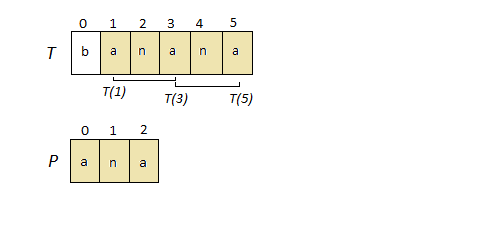
\includegraphics[width=0.4\textwidth]{1}
    \captionsetup{width=0.8\textwidth}
    \caption{The text $T$=\{banana\} and pattern $P$=\{ana\} over the alphabet $\Sigma$=\{abn\}. The pattern $P$ occours in $T$ in, at position $T[1]$ and $T[3]$. Notice that occurrences of $P$ may overlap.}
    \label{fig:banana}
\end{figure}
\newline
\\ 
Since most discussions of the exact string matching paradigm, begins with a naive method, this paper adobt the tradition, both presented by Gusfield et. al and by many others \cite{gusfield}. The naive method forms a basic understandig and insight to the more complex exact string mathing algorithms presented in the paper. 
\newline
The method align left end of $P$ with left end of $T$ and the scan from left to right, comparing characters of $P$ in $T$, until either there is a mismatch or $P$ is exhausted, in which case an occurence of $P$ in $T$ is reported. $P$ is then shifted one place to the right, and the character comparison is restarted from the left end of $P$ which repeats until $P$ shifts past right end of $T$ \cite{gusfield}.
\newline
Let $n$ denote the length of $P$ and let $m$ denote the length of $T$, then the worst-case timecomplexity of the naive method, is $\Theta$(nm). This is particular clear if $P$ and $T$ consists of the same repeated characters, such that the is an occurence of $P$ in $T$ for each of the first $m - n - 1$ positions.
\newline
Since most discussions of the exact string matching problem begin with the naive method. This paper adopt this tradition, as it form a basic insight to the more complex exact string matching algorithms presented later on \cite{gusfield}.
\begin{figure}[H]
    \centering
    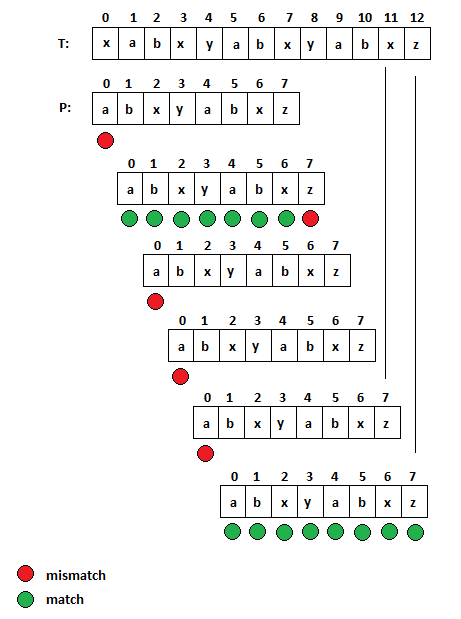
\includegraphics[width=0.4\textwidth]{comparisonbased1}
    \captionsetup{width=0.8\textwidth}
    \caption{The naive method, where $P$ is shifted one character to the right after each mismatch.}
    \label{fig:comparisonbased1}
\end{figure}

Let pattern $P$=  abxyabxz and let text $T$= xabxyabxyabxz.
\\ \\
Then the naïve method align left end of $P$  with left end of $T$ and scan from left to right, comparing the characters of $P$ with $T$, until either two disparate characters are located or $P$ is exhausted, in which case an occurrence of $P$ in $T$ is reported. If a character mismatch happens, $P$ is shifted one place to the right, until $P$ exceeds $T$, as illustrated in Figure \ref{fig:comparisonbased1} \cite{gusfield}.
The worst-case bound of the naïve method is $\Omega$(nm), which can be reduced to $\Omega$(n + m) with the basic idea of shifting $P$ more than one character at a time. This means that the number of character comparisons are reduced, due to $P$ moving through $T$ more rapidly. Some methods even exploit skipping over parts of the pattern after $P$ has shifted, further reducing character comparisons \cite{gusfield}. 
\begin{figure}[H]
    \centering
    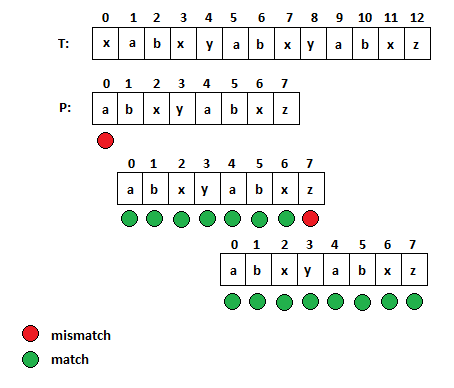
\includegraphics[width=0.4\textwidth]{comparisonbased2}
    \captionsetup{width=0.8\textwidth}
    \caption{After a mismatch, $P$ is shifted to the next occurrence of $a$ at position 5 in $T$, moving through $T$ more rapidly}
    \label{fig:comparisonbased2}
\end{figure}
\newline   
Figure \ref{fig:comparisonbased2}  illustrates the idea of shifting $P$ more than one character to the right. At initialization , the left end of $P$ aligns with left end of $T$, here comparing each character from $P$ with $T$ from left to right.
\newline
Let $P[0]$ denote the starting character of $P$ found at position 0, such that $P[0]=a$
\newline
\begin{figure}[H]
    \centering
    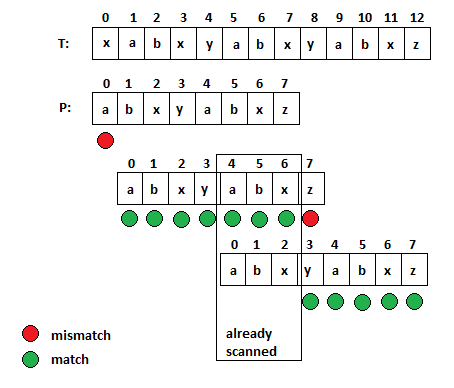
\includegraphics[width=0.4\textwidth]{comparisonbased3}
    \captionsetup{width=0.8\textwidth}
    \caption{Characters that have already been scanned are stored, so when $P$ is shifted to position 5 in $T$, $abx$ have already been scanned and can be skipped, and the character scanning is resumed from position 8 and 3, in $P$ and $T$, respectively.}
    \label{fig:comparisonbased3}
\end{figure}
When comparing characters, if a character in $T$ match $P[0]$, store the location. If a mismatch occur, shift $P$ to the stored location, here position 5 in $T$ and restart the character comparison, as in Figure \ref{fig:comparisonbased2}. This is doable for the reason that $P[0]=a$ does not occur in $T$ before position 5, such that $T[5]=P[0]=a$. 
The method in Figure \ref{fig:comparisonbased2} can be improved further, knowing that the next  three  characters are $abx$ after $P$ has shifted to position 5 in $T$. Knowing this, the first three characters are skipped, and character scanning are resumed from position 8 in $T$ and position 3 in $P$, as illustrated in Figure \ref{fig:comparisonbased3} \cite{gusfield}. 
\newline
The three methods presented exemplifies the basic idea of comparison based algorithms. More efficient algorithms have been developed, such as the Boyer-Moore and Knuth-Morris-Pratt algorithm, which have been implemented to run in linear time $(O(n+m) time)$ \cite{gusfield}. These are without a doubt interesting algorithms to analyze, however this paper merely delivers a short and precise description of the paradigm.
Another approach to the comparison based method is the preprocessing approach, where comparisons are skipped by first spending a small amount of time, learning about the internal structure of pattern $P$ or text $T$. Some methods preprocess pattern $P$ to solve the exact string matching problem, where the opposite approach is to preprocess text $T$, such as algorithms based on suffix trees \cite{gusfield}.

\subsection{Suffix trees}

The classic application for suffix tree is the substring problem \cite{gusfield, Kunihiko}, which is both a data structure -and an algorithmic problem \cite{mit}. That is, given a long text $T$ over some alphabet $\Sigma$, and some pattern $P$, the substring problem consist of preprocessing $T$ in linear time $O(m)$, and hereafter  $T$ should be able to take any unknown pattern $P$, and in linear time $O(n)$ determine occurrences of $ P$, if any, in $T$ \cite{gusfield}. The preprocessing time is here proportional to the length of text $T$, and the query is proportional to the length of pattern $P$ \cite{gusfield}. 
\newline
This paper adopts the approach of Gusfield et al., by not applying the denotation of pattern $P$ and text $T$, in respect to describing suffix trees. By using the general description and denotation of suffix trees, there will be less confusion, since input string can take different roles and vary for application to application \cite{gusfield}.
\newline
\newline
Conceptually a suffix tree is a compressed trie \cite{mit}.  
\begin{quote}
\textbf{Definition}    A trie contains all suffixes of string $S$, where each edge is labeled with a character from some alphabet $\Sigma$. Each path from root to leaf represent a suffix, and every suffix is represented with some path from root to leaf \cite{mit,Kunihiko}.
\end{quote}
\begin{figure}[h]
    \centering
    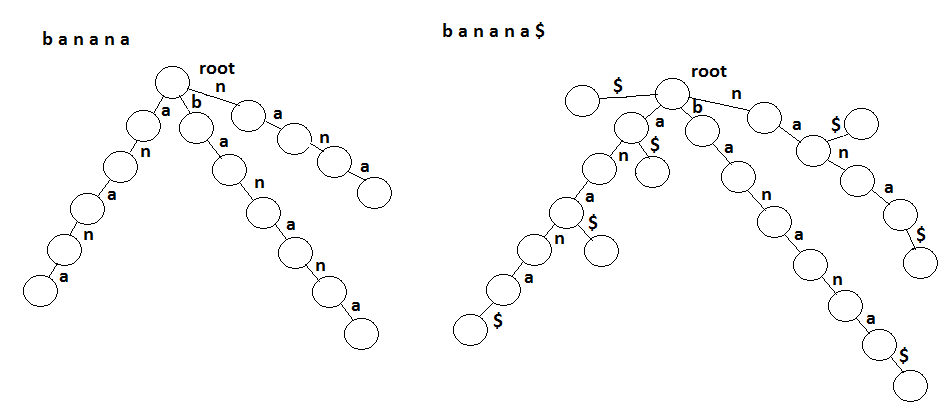
\includegraphics[width=0.6\textwidth]{trie}
    \captionsetup{width=0.8\textwidth}
    \caption{Left is a trie of the string $banana$ and the right is a trie of the string $banana\$$.}
    \label{fig:trie}
\end{figure}
\newline
Figure \ref{fig:trie} illustrates two tries, left of the string banana and the right over the string $banana\$$. Note that right trie has the termination character $\$$ appended to the end. This is due to the fact that the definition of a trie dictates that every suffix is represented with some path from root to leaf. Suffix $ana$ in left trie does not have a path from root to leaf, but appending a termination character to S that exists nowhere else in the string, will eliminate the problem.
\newline
Creating a compressed trie, one takes each non-branching nodes and compress them, such that edge-labels from non-branching nodes concatenates into a new edge-label, as illustrated in Figure \ref{fig:comprestrie}. Here node 1 is a non-branching node, one then concatenate a to n, to form a new edge-label na, deleting the non-branching node \cite{mit}. The number of non-branching nodes in a trie is at most the number of leaves. By compressing, we know have that the number of internal nodes is at most the number of leaves, having O(k) nodes total.
\newline

\begin{figure}[h]
    \centering
    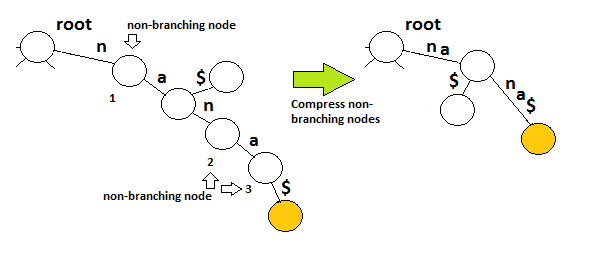
\includegraphics[width=0.6\textwidth]{compressingtrie}
    \captionsetup{width=0.8\textwidth}
    \caption{Compressing a trie.}
    \label{fig:comprestrie}
\end{figure}
\begin{quote}
\textbf{Definition}   A Suffix tree, $T$, is a $m$-character string $S$ concatenated with a termination character $\$$, that is represented as a directed rooted tree with exactly $m$ leaves, numbered $1$ to $m$. Except the root, each internal node contains at least two children, with each edge labeled with a nonempty substring of S. No two edges exiting a node can have labels beginning with the same character. The concatenation of edge-labels on the path from the root to leaf i, unerringly spells out the suffix of $S$ that starts at position i, such that it spells out $S[i..m]$. The termination character $\$$ is assumed to appear nowhere else in $S$, such that no suffix of the consequential string can be a prefix of any other suffix\cite{gusfield}.
\end{quote}
\begin{figure}[h]
    \centering
    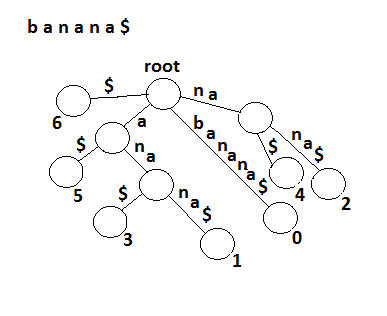
\includegraphics[width=0.4\textwidth]{suffixtree(banana)}
    \captionsetup{width=0.8\textwidth}
    \caption{A suffix tree $T$ for string $banana\$$.}
    \label{fig:suffixTree}
\end{figure}
The suffix tree for the string $banana\$$, in lexicographical order, is illustrated \ref{fig:suffixTree}. Each path from the root to a leaf $i$, unerringly spells out a suffix of $S$, starting at position $i$ in $S$. As an example, leaf numbered $2$ spells out $nana\$$, starting at position $2$ in the $S$, such that $S[2..6] = nana\$$. Each node has at least two children, and no two edges exiting a node begins with the same character. 
\newline
To dive into the substring problem using linear preprocessing time, $O(m)$, and linear search time, $O(n)$ we follow the tradition, and starts with a naive and straightforward algorithm to building suffix trees before verturing into the linear time preprocessing approach \cite{gusfield}. 

\subsection{Operations on suffix trees}

Bla bla bla...
\newline

\textbf{Insertion \& Deletion}
\textbf{Lowest Common Ancestor}

An interesting application of suffix trees is the $lca$ (Lowest Common Ancestor) problem, that is, finding the lowest common ancestor of node $i$ and $j$ in tree $T$. 
Lowest common ancestor was first obtained by Harel and Tarjan (1984, published online 2006 \cite{lcaWeb}) and later on simplified by Schieber and Vishkin (1988, published online in 2006 \cite{lcaWebSch})\cite{gusfield}.
\newline
Lowest common ancestor is an interesting application given that it is used in application as exact matching with wild cards and the $k$-mismatch problem, amongst others \cite{gusfield}. More interesting is the fact that $lca$ of leaves $i$ and $j$ identifies the longest common prefix of suffixes $i$ and $j$, which will be discussed later on.
\newline
By consuming linear time amount of preprocessing a suffix tree, that is a rooted tree, any two nodes can be identified and their $lca$ can be found in constant time, $O(1)$ \cite{gusfield, lca}. This paper will not dwell into the different linear time preprocessing algorithms for the $lca$ predicament, but delivers an overview and clarification of the problem by introducing a simpler but slower algorithm. (maybe linear in the appendix?).
\begin{quote}
\textbf{Definition}   In a rooted tree $T$ a node $u$ is an ancestor of node $v$, if $u$ is an unique path from the root to $v$ \cite{gusfield}.
\end{quote}
\begin{quote}
\textbf{Definition}   In a rooted tree $T$, the lowest common ancestor of two node $u$ and $v$, is the deepest node in tree $T$ that is an ancestor of both $u$ and $v$ \cite{gusfield}.
\end{quote}
Let’s suppose for simplification that an application is allowed preprocessing time of an upper bound of $\theta (n lg n)$, which is an acceptable bound for most applications \cite{gusfield}. Then, in the preprocessing state of tree $T$, perform a deept-first traversal of tree $T$ and create a list $L$ of nodes in order as they are visited. Then locating the $lca$ of node $2$ and $8$, $lca[2,8]$, in \cref{fig:travesal}, one only have to find any occurrences of $2$ and $8$ in $L$. Then take the lowest value in interval between $L[1] = 2$ and $L[12]=8$. This value is the lowest common ancestor for node $2$ and $8$ in $T$, $lca[2,8]=1$.
\begin{figure}[H]
    \centering
    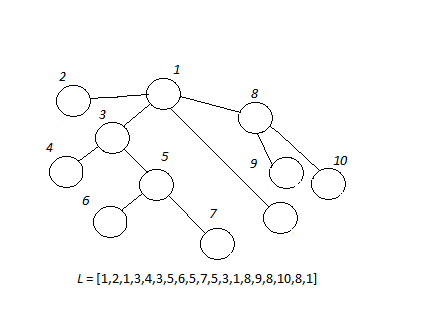
\includegraphics[width=0.5\textwidth]{travesal}
    \captionsetup{width=0.8\textwidth}
    \caption{Rooted tree - deept-first travesal with $L = [1,2,1,3,4,3,5,6,5,7,5,3,1,8,9,8,10,8,1]$}
    \label{fig:travesal}
\end{figure}


\textbf{Longest Common Prefix}

\begin{figure}[H]
    \centering
    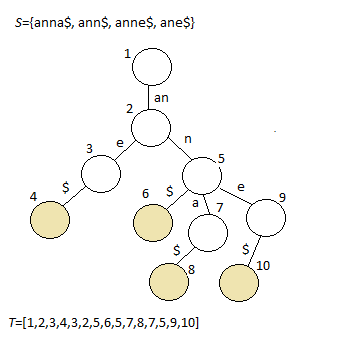
\includegraphics[width=0.4\textwidth]{suffixtree(speeling_anna)}
    \captionsetup{width=0.8\textwidth}
    \caption{Rooted tree - deept-first travesal with $L = [1,2,1,3,4,3,5,6,5,7,5,3,1,8,9,8,10,8,1]$}
    \label{fig:travesal_anna}
\end{figure}

What are the usages

\textbf{Predecessor $\&$ Successor Amongst Strings}

1 side

\textbf{Lowest Common Extension}

1 side

\subsection{Suffix Arrays}

Suffix array are space efficient alternatives to suffix trees \cite{gusfield,twoeffecient}. Before Manber and Meyers in 1990 introduced the first direct suffix array construction algorithm – SACA, suffix arrays were constructed using lexicographical-order traversal of suffix trees  \cite{gusfield,twoeffecient, performancesuffix, newapproach}. Manber and Meyers made suffix trees obsolete in respect to constructing suffix arrays, and their approach is known as a doubling algorithm, where with each sorting pass, doubles the depth to which each suffix are sorted. This means that suffixes are sorted in logarithmic number of passes, providing a worst case bound of $O(n log n)$ and $O(n)$ expected, assuming linear sort, reminiscent of Radix Sort \cite{performancesuffix} and queries can be answered in $O(P + log n)$ with use of Binary Search \cite{gusfield}.
\\
With the discovery of four different SACAs requiring only $O-(n)$ time worst case in 2003, the situation drastically changed. SACAs have since been the focus of intense research \cite{performancesuffix,newapproach}. In 2005 Joong Chae Na introduced more linear time SACAs, where two stood out, the Ko-Aluru (KA) algorithm for supplying good performance in practice and the Kärkkäinen-Sanders algorithm for its elegance \cite{newapproach}. 
\\
According to a survey paper, SACAs have to fulfill three important requirements: 
\begin{quote}
1. The algorithm should run in asymptotic minimal worst case time, where linear is an optimal way \cite{newapproach}. 
\end{quote}
\begin{quote}
2. The algorithm should run fast in practice \cite{newapproach}.
\end{quote}
\begin{quote}
3. The algorithm should consume as less extra space in addition to the text and suffix array as possible, where constant amount is optimal \cite{newapproach}.
\end{quote}
Although no current SACAs fulfill the requirements in an optimal way, research into faster and more space reducing SACAs continued \cite{newapproach}. Later on, in 2009, Nong et al. introduced two new linear time construction algorithms, one which outperformed most known and existing SACAs, called Suffix Array Induced Sorting SA-IS algorithm, guaranteeing asymptotic linear time and almost optimal space requirements \cite{newapproach}. 


\subsection{Suffix Trees To Suffix Arrays In Linear Time}







\subsection{SAIS - Suffix Array Induced Sorting Algorithm}

The SA-IS algorithm  is a divide and conquer and recursion algorithm, using variable-length leftmost S-type substrings and induced sorting \cite{twoeffecient}. In view of the fact that the SA-IS algorithm is unsophisticated to comprehend, implement and guarantees asymptotic linear time construction and close to optimal space,  SA-IS has been chosen as the single algorithm for the implementation of a malware detection system and the experiments which follow. 

\begin{quote}
\begin{lstlisting}[ basicstyle=\scriptsize, %or \small or \footnotesize etc.
]
SAIS(S, SA)
    (* Step 1 : Initialization & classification*)
    SA <-- suffix array of S
    t <-- type array
    P <-- LMS indicies array
    B <-- bucket array
    Scan S once from either left or right and classify all characters as 
        S-type or L-type and place them in t.
    Scan t once from  either left or right and locate all LMS substrings 
        in S and put them into P_1
    (* Step 2 : Induced sort LMS-substring)
    Induced sort all LMS substrings using P_1 and B
    Name each LMS substring in S by its bucket index to get a 
        new shortened string S_1
    (* Step 3 : Uniqueness - recursive step)
    (*@\textbf{if}  @*) T_1 is distinct, hence all characters are unique
       (*@\textbf{then}  @*) 
           Directly compute SA_1 from S_1
       (*@\textbf{else}  @*) 
           SAIS(S_1, SA_1)
    (* Step 4 : Induce SA from SA_1)
    Induce SA from SA_1       
    (*@\textbf{return}  @*) 
\end{lstlisting}
\end{quote}

\textbf{Basic notations}
\\ \\
Let $S$ be a string or text of $n$-characters stored in an array $[0…n-1]$ and let $\Sigma(s)$ be the alphabet of $S$. 
\\ \\
Let $S$$\$$ be a string $S$ concatenated with the termination symbol $\$$, where $\$$ is not contained in $S$ and is the lexicographical smallest character in $S$. For $S$ containing concatenation of multiple strings, let $S={S_0\$S_1\$...S_{n-1}\$}$, where $\$$ is the termination symbol for each concatenated string in $S$, and is the lexicographical smallest character in $S_0,S_1,...,S_{n-1}$. Furthermore, $S$ may not be contained in $S_0,S_1,...,S_{n-1}$. String $S$ is supposed to be concatenated with the unique termination symbol $\$$, if not explicit   stated otherwise \cite{twoeffecient}.
\\ \\
Let $suf(S,i)$ be some suffix in $S$ starting at $S[i]$ running to the termination symbol $\$$. $suf(S,i)$ is of S-type or L-type if $suf(S,i) < suf(S,i+1)$ or $suf(S,i) > suf(S,i+1)$, respectively \cite{twoeffecient}.
\\ \\
Let $suf(S, n-1)$ be the termination symbol and of S-type \cite{twoeffecient}.
\\ \\
Let $S[i]$ be S-type or L-type, if suf(S,i) is S-type or L-type, respectively \cite{twoeffecient}.
\\ \\
\textbf{Observation}
\begin{itemize}
  \item $S[i]$ is  S-type if $S[i] < S[i+1]$ or $S[i] = S[i+1]$ and $suf(S, i+1)$ is S-type \cite{twoeffecient}.
  \item $S[i]$ is  L-type if $S[i] < S[i+1]$ or $S[i] = S[i+1]$ and $suf(S, i+1)$ is L-type \cite{twoeffecient}.
\end{itemize}

The properties defined in the observation suggest that scanning from right to left, determing the type of each suffix or character can be done in constant time, $O(1)$, and that the type array $t$, can be filled in linear time, $O(n)$ \cite{twoeffecient}.

\begin{figure}[H]
    \centering
    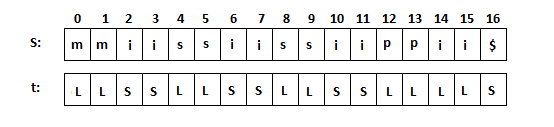
\includegraphics[width=0.6\textwidth]{SAISmmii1}
    \captionsetup{width=0.8\textwidth}
    \caption{Type array $t$ is filled from right to left}
    \label{fig:SAISmmii1}
\end{figure}

Figure \ref{fig:SAISmmii1} illustrates the filled type array, $t$, for text $S$=mmiissiissiippii\$, where text $S$ is scanned from right to left, determining the type of each suffix and character. Going from right to left in Figure \ref{fig:SAISmmii1} we have that $suf(S,16)$=\$ is a S-type, $suf(S,15)$=i\$ > $suf(S,16)$=\$ and is L-type, $suf(S,14)$=ii\$ > $suf(S,16)$=i\$ and is L-type and so forth, filling the type array $t$ in linear time.
\\ \\
Let $S[i]$ be a left most S-typeLMS character, if $S[i]$ is S-type and $S[i-1]$ is L-type, and let $suf(S,i)$ be a LMS suffix, if S[i] is a LMS character \cite{twoeffecient}.
\\ \\
Let $S[i..j]$ be a LMS substring if both S[i] and S[j] are LMS characters, and there exists no other LMS characters in the substring, and $i \neq j$ or it is the sentinel itself \cite{twoeffecient}.
\\ \\

\begin{figure}[H]
    \centering
    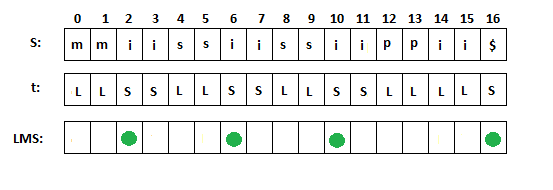
\includegraphics[width=0.6\textwidth]{SAISmmii2}
    \captionsetup{width=0.8\textwidth}
    \caption{Type array $t$ and LMS array defined for S=mmiissiissiippii\$}
    \label{fig:SAISmmii2}
\end{figure}

As Figure \ref{fig:SAISmmii2} exemplify, four LMS characters are defined for $S$=mmiissiissiippii\$, here at position 2, 6, 10 and 16 in $S$. Furthermore, four substrings and suffixes exists in $S$, namely $S[2..6]$, $S[6..10]$, S[10..16] and S[16..16], and $S[2..16]$, $S[6..16]$, S[10..16] and S[16..16], respectively.
After defining the S-types, L-types and LMS, the induction process of LMS substrings commence.
\\ \\

\textbf{Deffinition}
\begin{quote}
Determining the order of any two substrings, the corresponding characters are compared from left to right, comparing their lexicographical values first, and next their types, where S-type is considered highter priority than L-type \cite{twoeffecient}.
\end{quote}

\textbf{Induced sorting LMS substrings}
\\ \\
This part address the challenging problem of sorting the variable length LMS substrings. The basic idea is to create a new array, SA, and bucket sort the LMS substring into their equivalent buckets. Each bucket is named corresponding to the alphabet $\Sigma=\{\$,i,m,p,s\}$ in lexicographical order, such that SA contains four buckets, named $\$$, $i$, $p$ and $s$ in that order, as shown in Figure \ref{fig:SAIS_LMS} \cite{twoeffecient}.
$S$ is scanned from left to right, and indices for each LMS substring is appended to the end of its corresponding bucket in $SA$. The first LMS substring index is placed at the end of bucket for $i$, here at position 8 in $SA$ and forwards the bucket end one to the left, hence the bucket end for $i$ now rest at position 7 in $SA$. This process is repeated until all LMS substring indicies are placed in their buckets \cite{twoeffecient}.

\begin{figure}[H]
    \centering
    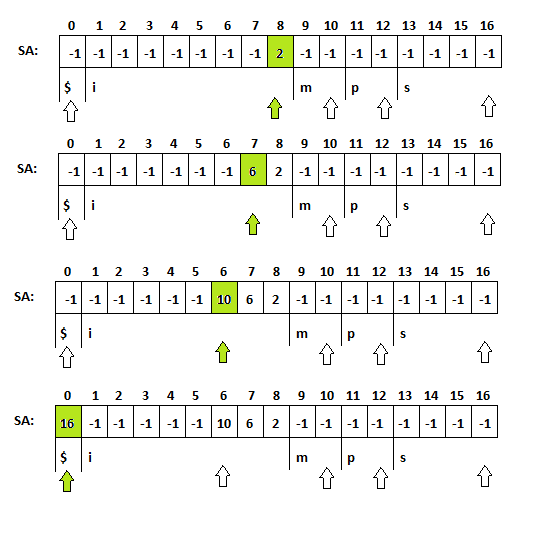
\includegraphics[width=0.5\textwidth]{SAIS_LMS}
    \captionsetup{width=0.8\textwidth}
    \caption{Induced sort of LMS substring}
    \label{fig:SAIS_LMS}
\end{figure}

When the LMS substrings are placed, then scan $SA$ from left to right and for each nonnegative value $S[i]$, if $S[i]-1$ is L-type, then place $SA[i]-1$ in the corresponding bucket for $suf(S, SA[i]-1)$, and lastly forward the bucket head one to the right \cite{twoeffecient}. 
\begin{figure}[H]
    \centering
    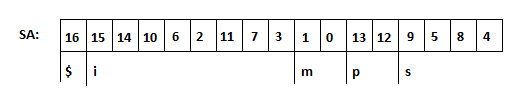
\includegraphics[width=0.5\textwidth]{SAIS_LMSfinal}
    \captionsetup{width=0.8\textwidth}
    \caption{$SA$ after the induced sorting for LMS substring.}
    \label{fig:SAIS_LMSfinal}
    
\end{figure}
\\
Roughly equivalent, when all L-types are placed, scan $SA$ from right to the left for each nonnegative value S[i], if $S[i]-1$ is S-type, then place $SA[i]-1$ in the corresponding bucket for $suf(S, SA[i]-1)$, and forward the bucket end one to the left. The above operations are demonstrated in Appendix \ref{SAIS Algorithm run} and the final result is displayed in Figure \ref{fig:SAIS_LMSfinal} \cite{twoeffecient}.
\\ \\
It is now the matter of determine if all LMS substrings are correctly sorted in SA, hence the uniqueness step in the SAIS algorithm. This is done by scanning $SA$ from left to right, and obtaining each LMS substring, and comparing the lexicographical values and types, and place them in buckets named accordingly to the lexicographical order they appear, starting from 0. So scanning from left to right in $SA$ given in Figure \ref{fig:SAIS_LMSfinal} gives the following bucket $B = \{\{0; \$\}, \{1; iippii\$\}, \{2; iissi, iissi\}\}$. The bucket keys are then placed in $S_1$ in the order as they appear in the original string $S$, hence $S_1 = \{2,2,0,1\}$ as illustrated in Figure \ref{fig:SAIS_LMSS}. If each character in $S_1$ is unique, hence does not exists any where else in $S$, then $SA_1$ can be computed directly from $S_1$, else fire the recursive step $SAIS(S_1, SA_1)$. $S_1$ for $S$ in Figure \ref{fig:SAIS_LMSS} is not distinct, since $2$ exists twice in $S_1$, hence $2$ is not unique, consequently a recursive step, $SA(S_1, SA_1)$,  is needed. Before venturing into the recursive step, save the original positions of the LMS substrings as they appear in $S_1$ into $P_1$, where $S_{1}[0] = 2$ points at position 2 in $S$,  $S_{1}[1] = 2$ points at position 6 in $S$, $S_{1}[2] = 1$ points at position 10 in $S$ and finally $S_{1}[3] = 0$ points at position 16 in $S$, such that $P_1=[2; 6; 10; 16]$ \cite{twoeffecient}.
\\
\begin{figure}[H]
    \centering
    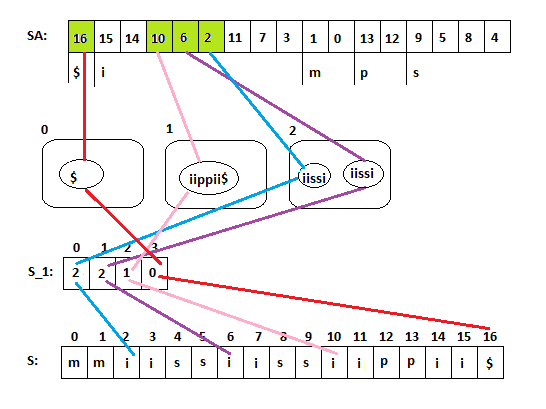
\includegraphics[width=0.5\textwidth]{SAIS_LMSS}
    \captionsetup{width=0.8\textwidth}
    \caption{Building $S_1$ from $SA$, using the original positions of the LMS substrings in $S$.}
    \label{fig:SAIS_LMSS}
    
\end{figure}
\\
In the recursive step for $SAIS(S_1, SA_1)$, locate S-types, L-types and LMS characters/substrings and determine if $S_1$ is distinct. In this case, as demonstrated in Figure  \ref{fig:SAIS_RECURSIVE}, there is only one LMS substring in $S$ so the new string $S_1$ is trivially distinct.
\\ \\
\textbf{Induce sort $SA$ from $SA_{1}$}
\\ \\
Either $SA_{1}$ has been computed directly from $S$ (if $S$ is distinct) or returned from one or more recursive steps. In either case, $SA$ can be induced sorted from $SA_1$ using information bound in $P_1$ \cite{twoeffecient}. 
\\ \\
First initialize all indicies in $SA$ with $-1$ and find the bucket ends. Then scan $SA_1$ from right to left and place $P_1[SA_1[i]]$ at the corresponding bucket end, and forward the bucket end one item to the left \cite{twoeffecient}. 
 \\
Then sort L-types by scanning $SA$ from left to right for each non-negative item $SA[i]$. If  $SA[i-1]$ is L-type, place $SA[i-1]$ in the corresponding bucket head for $SA$ and forward the bucket head one item to the right \cite{twoeffecient}.
\\
Last, sort all S-types by scanning SA from right to left for each non-negative item SA[i]. If  $SA[i-1]$ is S-type, place $SA[i-1]$ in the corresponding bucket end, and forward the bucket end one item to the left \cite{twoeffecient}. 
\\
\begin{figure}[H]
    \centering
    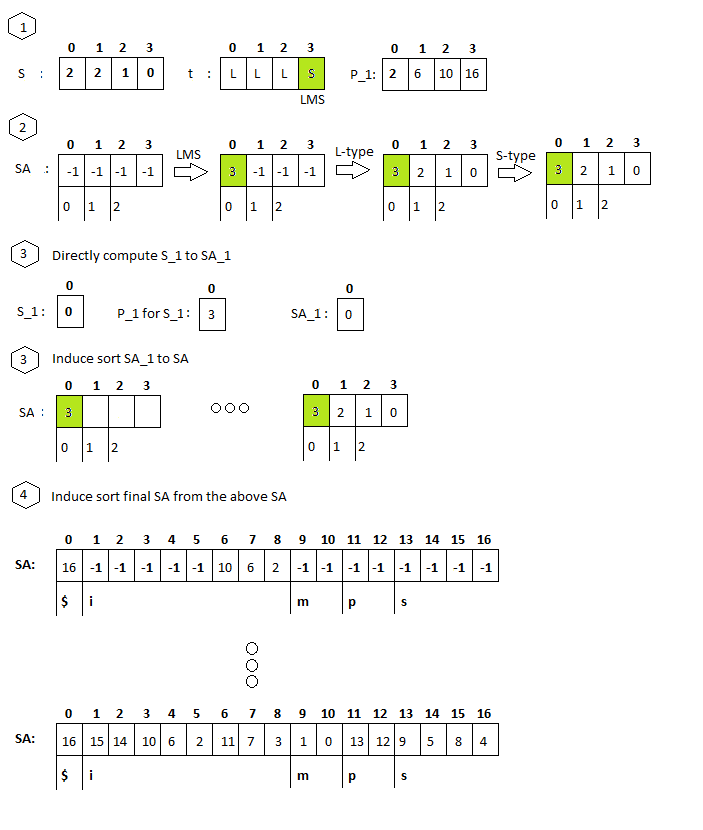
\includegraphics[width=1.0\textwidth]{SAIS_RECURSIVE}
    \captionsetup{width=0.8\textwidth}
    \caption{The recursive step $SA(S_1, SA_1)$.  First S-types, L-types and LMS characters/substrings for $S_1$ is localized. Secondly, induced sort LMS substrings, such that $SA_1 = [3;2;1;0]$. Last, scan $SA_1$ from right to left and place $P_1[SA_1[i]]$ into the buckets end of $SA$ as described for induced sorting LMS Substrings, for each item in $SA_1$. The final result is displayed in step 4.}
    \label{fig:SAIS_RECURSIVE}
    
\end{figure}
\\
This procedure is demonstrated in Figure \ref{fig:SAIS_RECURSIVEDESCRIPTION} where $SA$ is induced sorted from $S$ for the text $T$=mmiissiissiippii\$. SAIS returns the suffix array $SA$=[16; 15; 14; 10; 6; 2; 11; 7; 3; 1; 0; 13; 12; 9; 5; 8; 4] for text $T$=mmiissiissiippii\$ which is indeed sorted in lexicographical order as illustrated in Figure \ref{fig:SAIS_Sortedorder} \cite{twoeffecient}.
\\
It is now demonstrated how the algorithm works step by step. We now proceed to analyze the SAIS algorithm, here to insure that the algorithm actually returns a suffix array sorted in lexicographical order, for all legal inputs. Furthermore, the core mechanics of LMS-substring sorting is analyzed, giving a precise understanding of induce sorting LMSs, L-types and S-types. We will then prove correctness and completeness.

\begin{figure}[H]
    \centering
    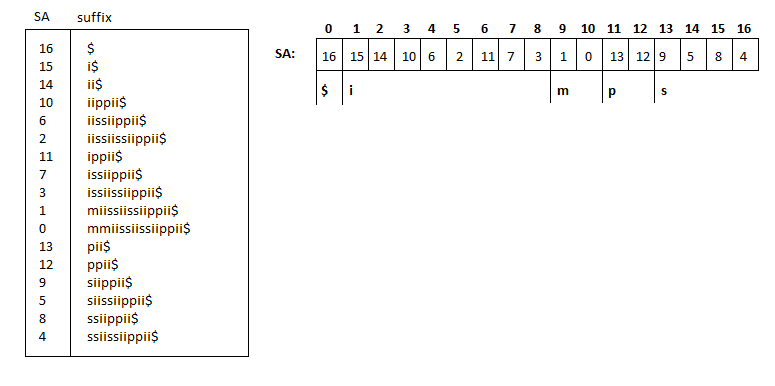
\includegraphics[width=0.6\textwidth]{SAIS_Sortedorder}
    \captionsetup{width=0.8\textwidth}
    \caption{The suffix array for the text $T$=mmiissiissiippii\$.}
    \label{fig:SAIS_Sortedorder}  
\end{figure}

\subsection{SAIS - Analysis, Correctness \& Completeness}
5-8 sider
\subsection{SAIS - Linear Time Preprocessing}
2 sider
\subsection{SAIS-FLS - Space requirement reduction for fixed length strings}

Suppose that string $S$ consists of fixed length strings concatenated together, where each string $S_0,S_1,...,S_{n-1}$ is terminated with the sentinel $\$$ such that $S=S_0\$S_1\$...S_{n-1}\$ $.
\\ \\
Let $S=S_0\$S_1\$...S_{n-1}\$ $ consist of concatenated fixed length distinct strings, such that $|S_0|$ = $|S_1|$=…=$|S_{n-1}|$ and each string in $S$ is terminated by the sentinel.
\\ \\
Let the length of pattern $P$, $|P|$, be same length as the fixed length distinct string in $S$, such that $|P|$=$|S_0|$ = $|S_1|$=…=$|S_{n-1}|$ .
\\ \\
Suppose that the string $S=jazz\$fuzz\$quiz\$$  is given and suffix array SA for $S$ has been computed, such that $SA=[14,4,9,1,5,12,0,10,11,6,13,3,8,2,7]$ as illustrated in Figure \ref{fig:jazz}.

\begin{figure}[H]
    \centering
    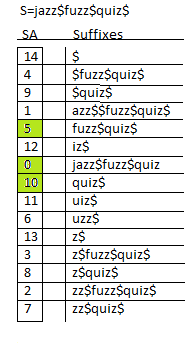
\includegraphics[width=0.2\textwidth]{jazz}
    \captionsetup{width=0.8
    \textwidth}
    \caption{Suffix array and suffixes for S=jazz$\$$fuzz$\$$quiz$\$$}
    \label{fig:jazz}
\end{figure}

By means of the Binary Search algorithm, suppose we want to find pattern $p_0=jazz\$$, $ p_1=fuzz\$$ and $p_2=quiz\$$ in the suffix array for $S$, such that $SA[i]$ pattern$ p_0=jazz\$$,$ p_1=fuzz\$$ must be a suffix of $T[SA[i]]$. Then $p_0=jazz\$$ is a suffix of $T[SA[0]]$, $p_0=fuzz\$$ is a suffix of $T[SA[5]]$ and $p_0=quiz\$$ is a suffix of $T[SA[10]]$. Now suppose, that we are only interested in exact matching, and do not care for unnecessary suffixes, then notice that we can match all fixed strings in $S$, with merely three indices in $SA$ for $S$, which leads to 12 indices in $SA$ for $S$ that are never used when exploiting exact string matching. 
\\
\begin{quote}
Let $N_DS$ denote the number of fixed length distinct strings in $S=S_0\$S_1\$...S_{n-1}\$ $, where $n$ is number of characters in $S$.
\end{quote}
\\ \\
This paper introduce an algorithm that reduce suffix array size for fixed length exact matching, from $O(n)$ to $O(N_DS)$ space complexity with linear time construction. 

\begin{quote}
\begin{lstlisting}
SAIS-FLS(string S, array SA, int len)
	let SA_FLS = new array[int]()
	for i=0 to i < length(SA) - 1 do:
		if(SA[i] NOT EQUAL TO length(S) - len
		&& S[SA[i] + len] EQUALS ''$'') 
			then PUT i in SA_FLS
	return SA_FLS
\end{lstlisting}
\end{quote}
\\
Describe the algorithm
\\
Some description here
\\

Analyzing the algorithm - something with loopinvariant
\\ 
\textbf{Initialization}
\\
Some description here
\\

\textbf{Maintenance}
\\
Some description here
\\

\textbf{Termination}
\\
Some description here
\\

\textbf{Correctness}
\\

Suppose that the length of the strings in $S$, $len$, is known, then scan $SA$ once, from left to right, and find any index where $T[SA[i] + len] = \$$ and add the elements to the new array SA-FLS in $O(m)$ time, where $m$ is the length of $SA$. Constructing the new suffix array for $S$ using SAIS-FLS, all unnecessary indices in SA are removed and the new array maintain the lexicographical order.
\\
\begin{quote}
\textbf{Lemma 6.9-1} $SAIS-FLS$ return a new array $SA-FLS$ that is sorted in lexicographical order.
\end{quote}
\\ \\
\textbf{Proof By Contradiction} 
\\ \\
Let $S$ be a string of strings, where each string is concatenated with the termination symbol $\$$. 
\\ \\
Let $SA$ be the suffix array for string $S$ and let $n$ denote the number of characters in $SA$. Suppose $SA$ is sorted lexicographical for all suffixes in $S$.
\\ \\
Suppose that S[SA-FLS[i]] to S[SA-FLS[j]], where i < j < |SA-FLS| is sorted in lexicographical order.
Suppose that $S[SA-FLS[j+1]]$ is lexicographical smaller than $S[SA-IS-FLS[j]]$, that would suggest that $SA$ for $S$ is not sorted lexicographical for all suffixes in $S$, which is a contradiction. Furthermore, since $SA$ is scanned from left to right and supposed sorted in lexicographical order, each item put in $SA-FLS$ must have been appended in lexicographical order. 
\\
\begin{quote}
\textbf{Lemma 6.9-2} $SAIS-FLS$ return a new suffix array, $SA-FLS$, containing all indices from $SA$ for $S=S_0\$S_1\$...S_{n-1}\$$ where $S[SA-FLS[i] + len] =\$$, $len = $|S_0|$ = $|S_1|$=…=$|S_{n-1}|\$$ and $0 < i < n$.
\end{quote}
\\ \\
\textbf{Proof By Contradiction} 
\\ \\
Suppose that there exist some $i$ and $j$, $i < j$, in SA, $0 < i < j < |SA|$ and $len = S_0$ in $S=S_0$$, $S_0$ =\$, where $S[SA[i] + len] = \$$ and $S[SA[j] + len] = \$$. Suppose that SA-FLS contain one item, that would suggest that $i=j$ which is a contradiction.
\\ \\
Suppose that $SA$ is sorted in lexicographically order for all suffixes in $S=S_0\$S_1\$...S_{n-1}\$$ where $S_0, S_1,…,S_{n-1}$ does not contain the termination symbol \$ and $len =|S_0|=|S_1|=…=|S_{n-1}|$.
\\ \\
Suppose that all indices from $SA$, where $S[SA[i]+ len] = \$$, $0 < i < n$, has been successfully added to the array $SA-FLS$. Suppose that there exists some $j$ in $SA-FLS$ where $S[SA-FLS[j] + len] =\$$, that would suggest that there exists an index $SA[i] = SA[j]$ where $S[SA[i] + len] =\$$, but that is a contradiction, since only indices that are bound by $S[SA-FLS[i] + len] =\$$ was added to $SA-FLS$.
\\ \\
Lemma 6.1-1 and Lemma 6.1-2 suggest that $SA-FLS$ contains indices in lexicographical sorted order and are bound by $S[SA-FLS[i] + len] =\$$. Furthermore, the length of $SA-FLS$ is proportional to the number of the fixed length distinct string in $S=S_0\$S_1\$...S_{n-1}\$$.
For large fixed length strings such as SHA1, SHA256 or MD5 hashes, $SA-FLS$ concededly reduce the number of indices stored. A string consisting of 27.000.000 MD5 hashes would produce a suffix array consisting of 27.000.000 x 33 = 891.000.000 indices, while SA-FLS contains only 27.000.000 indices, which is a reduction factor of 33. For the Sha256, the reduction factor would be 257, hence the length of the hash plus the termination symbol.

\begin{figure}[H]
    \centering
    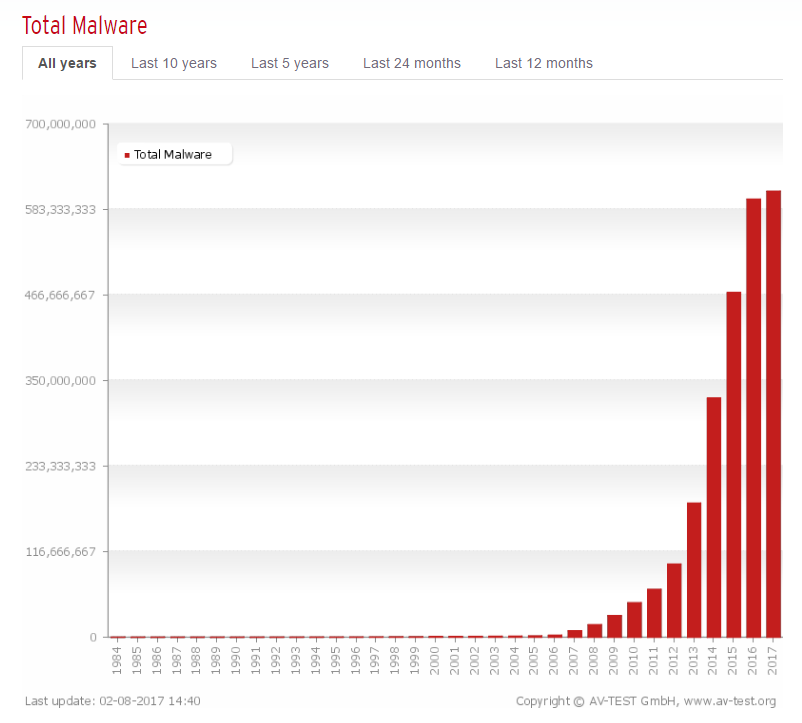
\includegraphics[width=0.6\textwidth]{totalmalware}
    \captionsetup{width=0.8\textwidth}
    \caption{According to AV-TEST, an independent IT-security institute https://www.av-test.org/en/statistics/malware/, 390.000 new malicious programs are identified each day, bringing the total malware count obove 580.000.000 for 2017.}
    \label{fig:totalmalware}
\end{figure}

\subsection{Burrows-Wheeler Transform}
\subsection{SAIS-OPT - Optimization of the SA-IS Algorithm using Burrows-Wheeler Transform}
2-3 sider

\section{Malware - Malicious Software}

- Encryption
- Do md5 ganrantee uniqueness?

\subsection{Building database of known malware - MD5 encryption}

\section{Malware Detection System - An exact string matching approach}
\subsection{Building interactive systems - Windows (R) Forms}

- Approach
- Investigation and project planning

\subsection{Database - RAM vs HHD}
\subsection{Network & security}

\section{Evaluation and recommendations}

\section{Discussion}

\section{Future work}

\section{Conclussion}
\section{Literature list and references}
\section{Appendix}



%-----------------------------------------------------------------------------

%-----------------------------------------------------------------------------
\newpage
\appendix
\label{appendix}
\section{SAIS Algorithm run}\label{SAIS Algorithm run}
\begin{figure}[H]
    \centering
    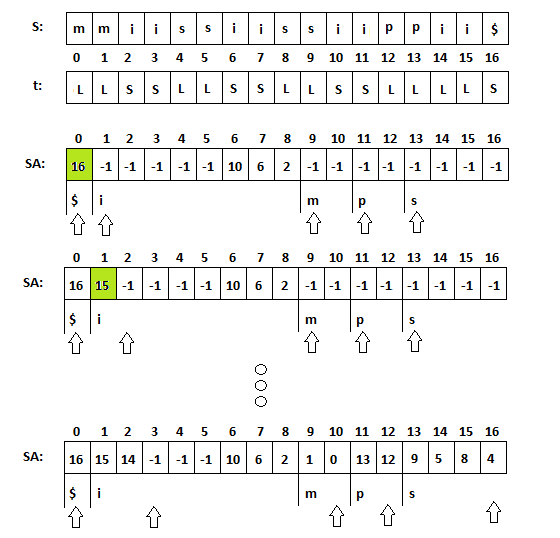
\includegraphics[width=0.5\textwidth]{SAIS_LMS2}
    \captionsetup{width=0.8\textwidth}
    \caption{$S$ is scanned from left to right, and indices for each LMS substring is appended to the end of its corresponding bucket in $SA$. The first LMS substring index is placed at the end of bucket for $i$, here at position 8 in $SA$ and forwards the bucket end one to the left, hence the bucket end for $i$ now rest at position 7 in $SA$. This process is repeated until all LMS substring indicies are placed in their buckets.}
    \label{fig:SAIS_LMS2}
\end{figure}
\begin{figure}[H]
    \centering
    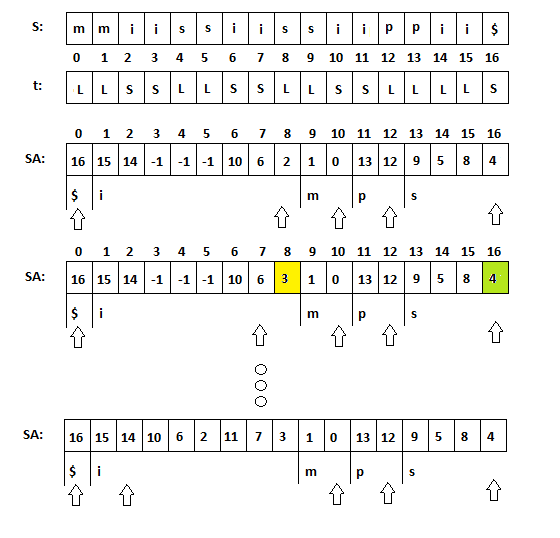
\includegraphics[width=0.5\textwidth]{SAIS_LMS3}
    \captionsetup{width=0.8\textwidth}
    \caption{$S$ is scanned from left to right, and indices for each LMS substring is appended to the end of its corresponding bucket in $SA$. The first LMS substring index is placed at the end of bucket for $i$, here at position 8 in $SA$ and forwards the bucket end one to the left, hence the bucket end for $i$ now rest at position 7 in $SA$. This process is repeated until all LMS substring indicies are placed in their buckets.}
    \label{fig:SAIS_LMS3}
\end{figure}
\lipsum[21]
%I will let this talk for it self. And no, you don't need it right now, so out comment it or delete it $\ddot\smile$
\newpage
\section{SAIS Recurssive step}\label{SAIS Algorithm run}
\begin{figure}[H]
    \centering
    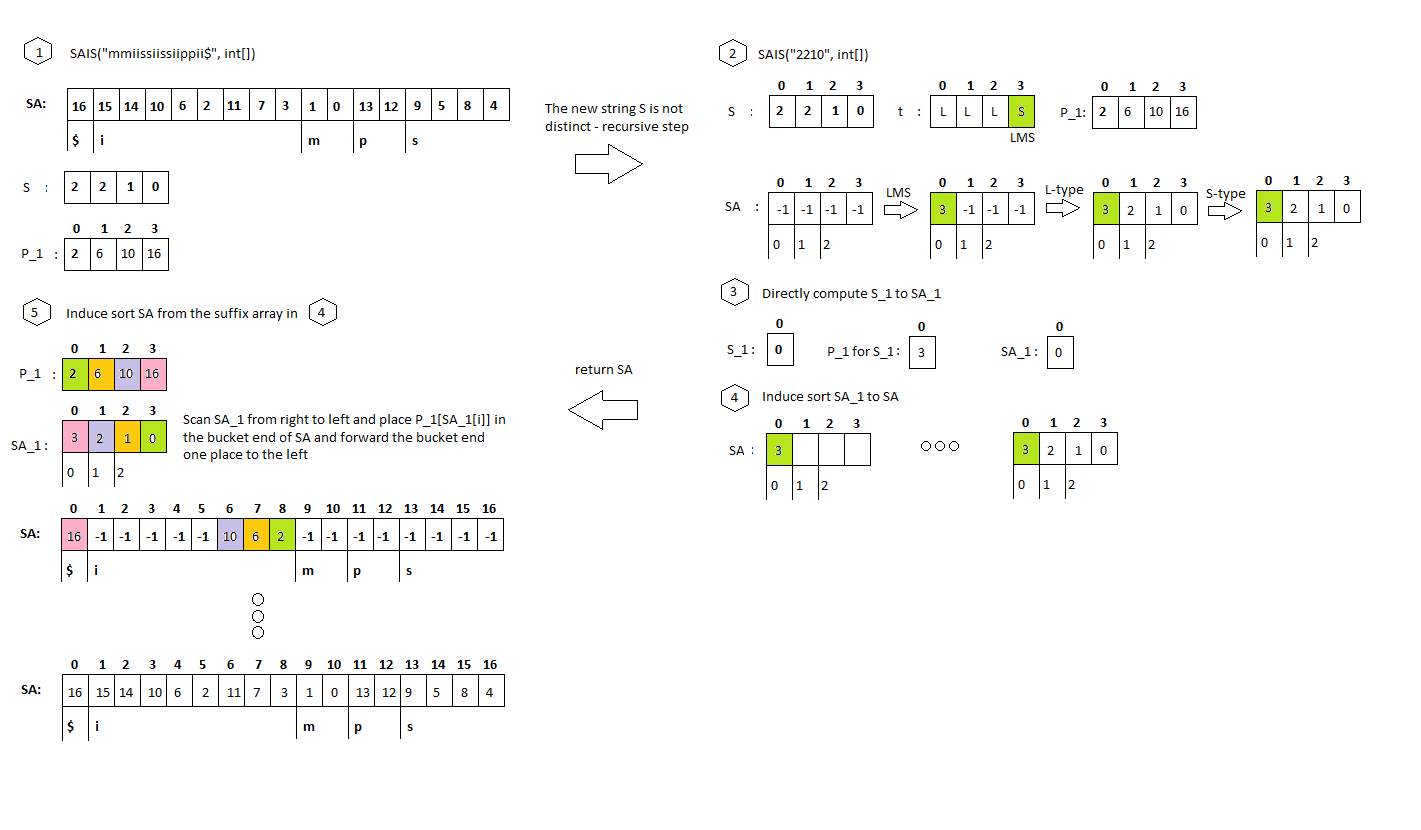
\includegraphics[width=1.1\textwidth]{SAIS_RECURSIVEDESCRIPTION}
    \captionsetup{width=0.8\textwidth}
    \caption{Some description here}
    \label{fig:SAIS_RECURSIVEDESCRIPTION}
\end{figure}

% THIS I WILL NOT EXPLAIN RIGHT NOW - WE CAN TAKE IT WHEN IT IS MORE RELEVANT!
\newpage
\nocite{*}
\bibliographystyle{ieeetr}
\bibliographystyle{unsrt}
\bibliography{bibliography}
%-----------------------------------------------------------------------------
\end{document}